\chapter{Introduction}\label{introduction}
Dialogue system (i.e. conversational agent) is a computer system which interacts with a human in natural language. These systems are used in cars (hands-free car-specific functions, Android Auto, Apple CarPlay), web, robots, computer games etc, because a conversation is a natural way for people to get information. 

Natural Language Generation (NLG) is an important component of dialogue systems, which has a significant impact on system quality, because NLG goal is to imitate human behaviour. The conversational agent can be classified into task-oriented (i.e. goal-oriented), which focused on completing a certain tasks and adhere to a determined script for each stage of the conversation, and non-task-oriented, which do not have a stated goal to work towards. A lot of devices have incorporated goal-oriented dialogue systems, such as Yandex’s Alisa, Apple’s Siri, Microsoft’s Cortana, Amazon Alexa, and Google Assistant. Goal-oriented dialogue acts make conversations more interpetable and controllable. On the other hand, they also hinder scaling such systems to new domains (i.e. conversation topics). To escape from the limitation, recent interest of research started moving to non-task-oriented chitchat dialogues (chatbots). Chitchat dialogues are systems designed to mimic the unstructured human-human conversation. This kind of conversational agent often have an entertainment value, such as Cleverbot, Microsoft's XiaoIce system etc. Chatbots have also been used for testing theories of psychological counseling.

The ability to communicate freely in a natural language is one of the hallmarks of human intelligence, and is likely one of the requirements for true artificial intelligence. Many researches work on open-ended (i.e. there is a huge range of appropriate outputs given the input) chitchat dialogues to explore this aspect of intelligence, because in goal-oriented dialogue systems there is a relatively narrow range of correct outputs given the input. 
Creating a non-task-oriented agent is a challenge for researches, because there are a lot of topics of conversations as well as user reactions and responses to them. Such bots are not able to generate meaningful conversations. Their replies are often too generic, because non-specific responses sound quite natural (e.g. ``Ok, I see'', ``I don't know''). There are still a lot of problems in the Natural Language Generation, such as response-relatedness, semantic errors, repetition etc., which will be described in more detail in the chapture \ref{nlg_problems}. 

According to \cite{salovey1990emotional} one of the most important cognitive behaviors in humans is expressing and understanding emotions. That is why it is necessary to pay attention not only to generation of a semantically and syntactically correct text, but also to the emotions and language style in which person communicates to make a dialogue more diverse and interesting. Carefully formulated speech without cliches or jargon is essential to avoid inaccurate presentation and ensure effective communication. Most of the modern generative models are trained on huge corpora which include different contributions from various authors. Texts produced with such models are often not perceived as natural and characterized as non-human, because humans have recognizable writing and communication styles.


The main purpose of this thesis was to create NLG model, which will be able to generate text in different styles.  //TODO


\chapter{NLG problems in dialogue systems}\label{nlg_problems}
In a book \cite{alder2017handbook} Natural Language Generation is defined as ``the process by which thought is rendered into language''. NLG approaches can be grouped into two categories, one focuses on generating text using templates or (linguistic) rules (i.e. data-to-text generation), the other uses corpus-based statistical methods (i.e. text-to-text generation), where corpora is a collection of texts \cite{oh2002stochastic}.


\begin{figure}[hbt]
  \centering
  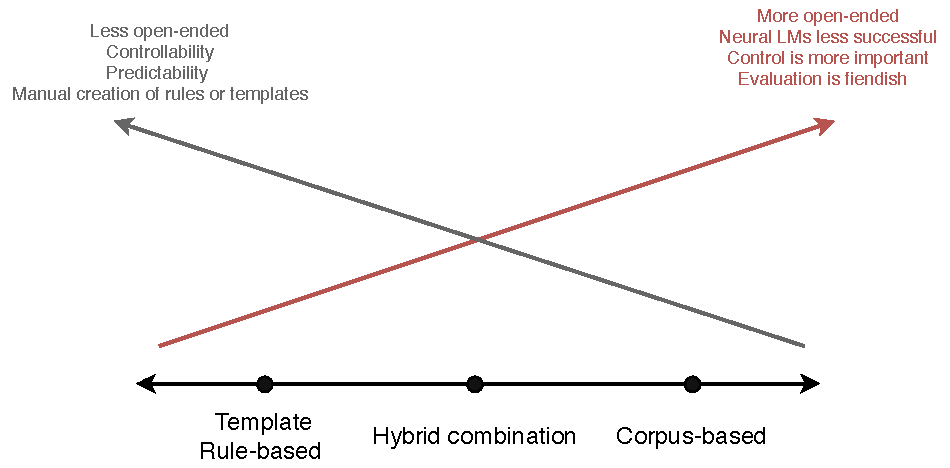
\includegraphics[width=0.9\textwidth]{figures/templateVScorpus.pdf}
  \caption{Spectrum of the NLG tasks.}
  \label{nlg_spectum}
\end{figure}

\section{Template-based approach} 

\begin{table}[ht]
\centering
 \begin{tabular}{|c|} 
 \hline
 Example: \\
 \hline
 User's input: \\
 ``I'm going to travel from Moscow on April 2.'' \\ 
 \hline
 Template: \\
 What time would you like to travel from $\{departure\_city\}$ on $\{departure\_date\}?$ \\
 \hline
 Agent's output:\\
 ``What time would you like to travel from Moscow on April 2?'' \\
 \hline
 \end{tabular}
 \caption{The example of template-based approach.}
\label{tab:tb_example}
\end{table}

Until recently Natural Language Generation component of a dialog system used primarily hand-coded generation templates, which represented model sentences in a natural language mapped to a particular semantic content.
The template-based system selects a proper response for the current conversation from a repository with response selection algorithms. Templates are often designed for a specific task in a given domain \cite{manishina2016data}. 
Example of template-based system is shown in the Table \ref{tab:tb_example}.


\subsubsection{Advantages of template-based approach}
The output produced by this approach is likely to be grammatically correct and not contain unexpected generation errors. The process of sentence generation is fully controlled, these models are robust and reliable because they consist of clearly defined rules. 

\subsubsection{Disadvantages of template-based approach}
These models require time and human resources to deploy a real dialogue system, because templates are constructed manually, and the number of templates grows quickly (using different templates for singular and plural versions). These systems are not able to handle unknown inputs. Templates often sound unnatural due to their generic structures. Template-based systems cannot make variation in output, it is just concatenation of strings. This approach is not flexible, because it has limits to use templates in other domains. Template-based model is not able to learn and is not able to adapt to the user, that's why it generates rigid and stylised responses without the natural variation of human language.

\section{Corpus-based approach}
Corpus-based system dominates the NLG community, special in the case of open-ended tasks, where it is almost impossible to hand-craft the templates for all possible combinations of semantic units. Corpus-based systems include statistical and machine learning approaches to resolve it \cite{rudnicky2002dialog}.

One of the first approaches in corpus-based methods is \textbf{Dynamic Sentence Generation}, which dynamically creates sentences from representations of the meaning to be conveyed by the sentence and/or its desired linguistic structure. It allows do not write code for every boundary case and includes aggregation, reference, ordering and connectives to optimise sentences.

Next level of corpus-based approaches is \textbf{Dynamic Document Creation}, what can produce relevant and well-structured document. 

\subsubsection{Advantages of corpus-based approach}
Corpus-based models have ability to generate more proper responses that could have never appeared in the corpus; it is possible to mimick the language of a real domain expert and use this models for open-domain dialogue systems; dynamic approach is able to learn and to handle unknown inputs, it is also has a lot of possible variations of output.

\subsubsection{Disadvantages of corpus-based approach}
It is necessary to have a corpus, which contains a large amount of data and on a variety of topics to get a sensible output. Even if you have the corpus, process of text generation is not fully controlled and the output can be incorrect or does not make a sence. This approach still has a lot of problems, what will be described in more detail in the section \ref{nlg_ds_problems}. 

\section{Language Models}
In corpus-based system natural language generation uses \textbf{Language Models(LMs)} to generate sequences of texts. LM is a probabilistic model which learns to predict the probability of a sequence of words. The equation \ref{eq:LM} represents the language model, where $W$ is a sequence and $w_1, w_2, ..., w_n$ are words in this sequence. The language model provides a context for distinguishing words and phrases that sound the same. For example the phrases ``but her'' and  ``butter'' sound the same, but mean different things.

\begin{equation} \label{eq:LM}
P(W) = P(w_1, w_2, ..., w_n)
\end{equation}

The \textbf{Chain rule} (equation \ref{eq:CR}) is used to calculate the joint probability of a sentence by using the conditional probability (equation \ref{eq:CB}) of a word given previous words. 
\begin{equation} \label{eq:CR}
P(w_1, w_2,..., w_n) = \prod_{i}P(w_i|w_1, w_2,...,w_{i-1})
\end{equation}

\begin{equation} \label{eq:CB}
P(A|B) = P(A \cap B) / P(B)
\end{equation}
In equation \ref{eq:CB} $P(A \cap B)$ is the probability that both events A and B occur.

\begin{figure}[hbt]
  \centering
  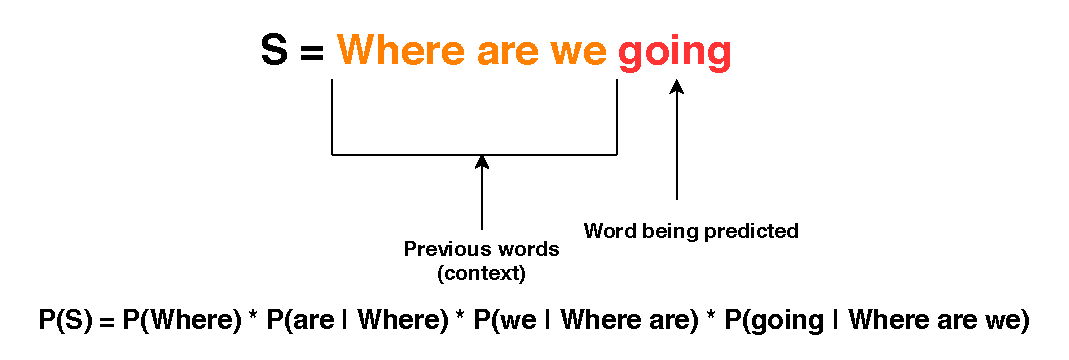
\includegraphics[width=0.8\textwidth]{figures/lm.pdf}
  \caption{Example of a word prediction by using chain rule.}
  \label{chain_rule}
\end{figure}

An example in the Figure \ref{chain_rule} shows how to predict probability of a word given previous words. A subsequence (context) may consist of a very large number of words and the likelihood that such subsequence is found in a corpus is very small. It is a main problem in language models, which is called \textbf{data sparsity}.

Data sparsity is the phenomenon of not observing enough data in a corpus to model language accurately. The solution to resolve this issue is to make the assumption that the probability of a word depends only on the previous \textit{n} words and use \textbf{N-gram model} (N-gram is a sequence of N words).

\begin{table}[ht]
  \centering
   \begin{tabular}{|c|c|} 
   \hline
    Hi & 1-gram \\
   \hline
    New York & 2-gram \\
   \hline
   The Three Musketeers & 3-gram \\
   \hline
   She is studying IT & 4-gram \\
   \hline
   \end{tabular}
   \caption{The example of N-grams.}
  \label{tab:n_gram}
\end{table}

The n-gram ``She is studying IT'' from the Table \ref{tab:n_gram} does not occur as often in texts of corpus as n-grams ``Hi'', ``New York'' and ``The Three Musketeers''. Knowing a probability to the occurrence of an N-gram in a sequence of words can be useful, because it can help to decide which N-grams can be chunked together to from single entities (like ``New York'' chuncked together as one word). It can also help make next word predictions. For example, ``tea'' is more likely than ``ball'' in the phrase ``I would like to drink''.


According to \cite{bengio2003neural} another way to fight with data sparsity is learning a distributed representation for words, which allows each training sentence to inform the model about an exponential number of semantically neighboring sentences. The model learns simultaneously a distributed representation for each word along with the probability function for word sequences. A sequence of words that has never been seen before gets high probability if words in this sequence are similar in the sense of having a nearby representation to words forming an already seen sentence. Authors used neural networks (artificial neural networks are described in the section \ref{nn_section}) for the probability function. The proposed approach improved n-gram models and took an advantage of longer contexts.


\section{Dialogue systems}\label{nlg_ds_problems}
The ability to communicate with machines in a natural language is a long-standing dream of mankind. Today's dialogue systems often encounter criticism. There are many scientific works on creating more natural dialogue systems. Markus M. Berg defines a natural dialogue system in \cite{berg2014modelling} as ``a form of dialogue system that tries to improve usability and user satisfaction by imitating human behaviour''. It affects the features of human-to-human dialogue (for example, topic changes, sub-dialogues) and seeks to integrate them into dialogue systems for human interaction with the machine. Open-ended natural dialogue systems still have flaws in generating a response to the user.

\begin{table}[ht]
\centering
 \begin{tabular}{|p{0.5cm}|p{8cm}|} 
 \hline
 1 & More phones have games on them than this one. \\
 \hline
 2 & Why a mouse when it spins? \\
 \hline
 \end{tabular}
 \caption{A problem of adequacy shows that a response can be grammatically and syntactically composed correctly, but this sentence does not make sense.}
\label{tab:adequacy_prob}
\end{table}

\begin{table}[ht]
\centering
 \begin{tabular}{|p{0.5cm}|p{8cm}|} 
 \hline
 1 & They IS going to school. \\ 
 \hline
 2 & It depends AT you. \\
 \hline
 \end{tabular}
 \caption{A problem of syntactic correctness.}
\label{tab:syntactic_corr_prob}
\end{table}

\begin{table}[ht]
\centering
 \begin{tabular}{|c|} 
 \hline
  -Yes, I'm studying law at the moment.\\
  - Good. \\
  - I like playing the piano. \\
  - Good. \\
 \hline
 \end{tabular}
 \caption{A problem of repetition makes conversation boring.}
\label{tab:repetition_prob}
\end{table}

\begin{table}[ht]
\centering
 \begin{tabular}{|c|} 
 \hline
 -Do you go get coffee often? \\
 -I am a musician. \\
 \hline
 \end{tabular}
 \caption{A problem of response-relatedness shows that the answer to the question does not make a sense in this context and it spoils the impression of the conversation.}
\label{tab:response_relatedness_prob}
\end{table}

As noticed in \cite{stent2005evaluating}, the main task of NLG is to select, inflect and order words ``to communicate the input meaning'' as completely, clearly and fluently as possible in context. That's why it is necessary to control not only syntactic correctness of output but also if output is appropriate or felicitous in a given context. A good generator usually relies on several factors:
\begin{itemize}
  \item \textbf{adequacy} (a sentence that is ambiguous or not contains communicates meaning in the input, is \textbf{not} adequate (an example in the Table \ref{tab:adequacy_prob}))  
  \item \textbf{syntactic correctness} (an example in the Table \ref{tab:syntactic_corr_prob})
  \item \textbf{repetition} (self-repetition across utterances and with utterances, repeating the conversational partner (an example in the Table \ref{tab:repetition_prob}))
  \item \textbf{response-relatedness} (efficacy in context (an example in the Table \ref{tab:response_relatedness_prob}))
  \item \textbf{variation} (there are 2 basic forms of variation: \textit{word choice variation} and \textit{word order variation} for enriching speech)
\end{itemize}

\begin{table}[ht]
\centering
 \begin{tabular}{|p{0.5cm}|p{8cm}|} 
 \hline
 \# & Example \\
 \hline
 1 & I bought movie tickets on Tuesday. \\ 
 \hline
 2 & I got movie tickets on Tuesday. \\
 \hline
 3 & On Tuesday I bought movie tickets. \\
 \hline
 4 & On movie Tuesday tickets I bought. \\
 \hline
 5 & I bought tickets for the Tuesday movie. \\ 
 \hline
 \end{tabular}
 \caption{The example of sentences' variation.}
\label{tab:var_example}
\end{table}

An example in the Table \ref{tab:var_example} shows all types of variation. Sometimes this factor can be syntactically incorrect or unclear, what you can see in the forth sentence. In fifth sentnecne a variation changed the meaning of part of the sentence. In addition, the variation may add or remove meaning possibilities.


One of the hardest problem in text generation is a language style, which makes a response to an user more human. This task is challenging due to the difficulty of capturing emotional factors and the complex mechanism of human emotions. Some people use obscene speech, some use a lot of expressive means, jargon or jokes to make speech more emotional. This is what distinguishes people and makes their communication more interesting.

\chapter{Models for Natural Language Generation}
NLG evolution from templates to dynamic generation of sentences took a lot of time and models developed along with it. Corpus-based generation uses a generative probabilistic model what can be implemented in many ways. The model focuses on response generation in the context of dialogue, where the task is to generate a response, given an utterance. Thus, these models fit well within the sequence-to-sequence (seq2seq) (i.e. encoder-decoder) models with using neural networks (NNs), which are described in more detail in section \ref{seq2seq_section}, but first a short description what neural networks are, for a better understanding seq2seq model.

\section{Neural Networks} \label{nn_section}
Artificial Neural Networks are inspired by biological neural networks that constitute animal brains. Artificial neuron (on the Figure \ref{neuron}) is a computational unit in an artificial neural network with a set of real-valued inputs $x_1, x_2 ... x_n$ and an output $y$, where each input $x_i$ has a corresponding weight $w_i$. Weights determine the influence of the input on the output. The neuron's output is the weighted sum of its inputs, which are passed through a non-linear function known as an activation function or transfer function. The transfer functions usually have a sigmoid shape and model the threshold for neuron firing. Bias is an additional parameter in the Neural Network, which is used to adjust the output along with the weighted sum of the inputs to the neuron. Bias value allows to shift the activation function either right or left.

\begin{figure}[hbt]
  \centering
  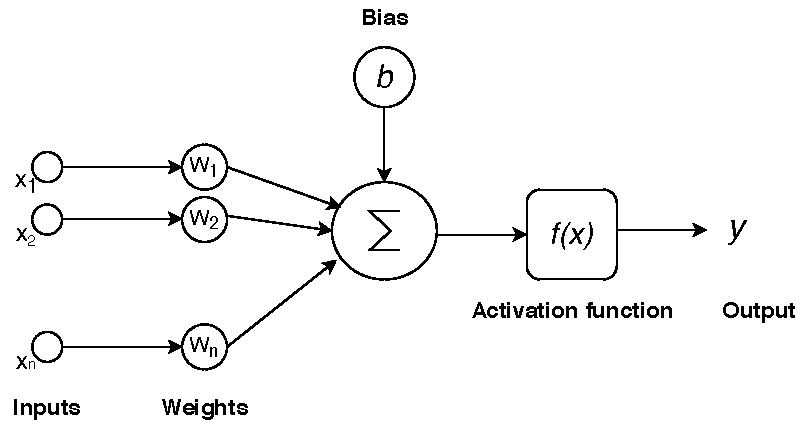
\includegraphics[width=0.5\textwidth]{figures/ai_neuron.pdf}
  \caption{Architecture of an artificial neuron.}
  \label{neuron}
\end{figure}

\begin{figure}[hbt]
  \centering
  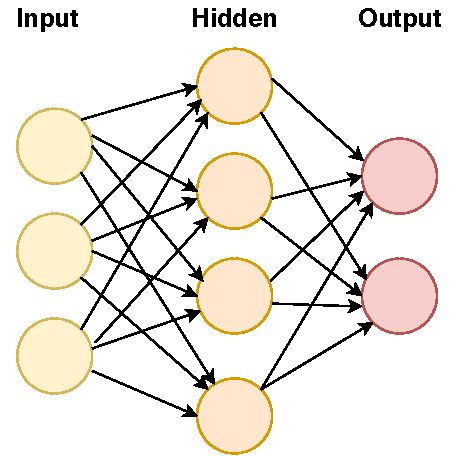
\includegraphics[width=0.3\textwidth, height=0.2\textheight]{figures/nn.pdf}
  \caption{The fully-connected neural network with 1 hidden layer.}
  \label{nn}
\end{figure}

Neural networks are acyclic directed graphs of neurons. Neurons' outputs can be connected to inputs of other neurons and the calculation is propagated through the network. In NNs neurons are organized into layers where generally the output of the layer is the input for a next layer. The Figure \ref{nn} represents the most common type of layer - the fully-connected layer where all neurons between adjacent layers are connected with each other.

\section{Recurrent neural network (RNN)} \label{rnn_section}
Recurrent neural networks are a special type of a neural network used in natural language processing(NLP) as they allow temporal depedencies in the data (like context) to be captured. RNNs share the same structure as NNs described in the section \ref{nn_section}, except each layer also has an internal state (i.e. hidden state), which captures information about the previous layer inputs. This allows the network to keep track of past data while processing current inputs.

\begin{figure}[hbt]
  \centering
  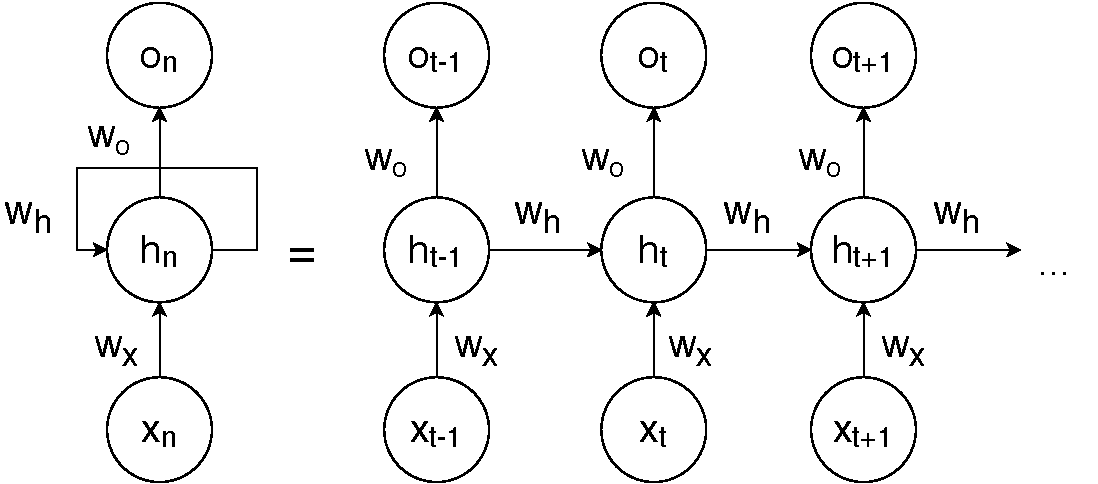
\includegraphics[width=0.5\textwidth]{figures/rnn.pdf}
  \caption{Architecture of a recurrent neural network, where coefficient \textbf{h} is a hidden state, \textbf{x} is an input and \textbf{o} is an output. Coefficient \textbf{w} is a weight, what is transformed to produce a sensible output.}
  \label{rnn}
\end{figure}


The architecture of RNN is illustrated in the Figure \ref{rnn}. A hidden state $h$ is realized as a vector, which calculated from the input $x$ and the previous hidden state. An output $o$ is calculated from this new hidden state. 
The equations \ref{eq:rnn_h} and \ref{eq:rnn_o} show the formulas for a traditional recurrent neural network.
\begin{equation} \label{eq:rnn_h}
h_t = \sigma(W_hh_{t-1} + W_xx_t)
\end{equation}

\begin{equation} \label{eq:rnn_o}
o_t = softmax(W_oh_t)
\end{equation}

The RNN-based models have been used for NLG as a component of end-to-end trainable goal-oriented dialogue system \cite{wen2016network} and a training model with semantic aggregation \cite{tran2017neural}. 

Nowadays traditional RNN networks almost are not used in NLG, because they have problems with vanishing and exploding gradients. As introduced in \cite{bengio1994learning} the exploding problem refers to the large increase in the norm of the gradient during training. It happens, because long term components can grow exponentially more then short term ones. The vanishing gradients problem refers to the opposite behaviour. The long term components go exponentially fast to norm 0, which makes it impossible for the model to learn correlation between temporally distant events. This issue has motivated researchers in development of more advanced RNNs like the LSTM \cite{hochreiter1997long}.

\section{Long short-term memory (LSTM)} \label{lstm_section}

\begin{figure}[hbt]
  \centering
  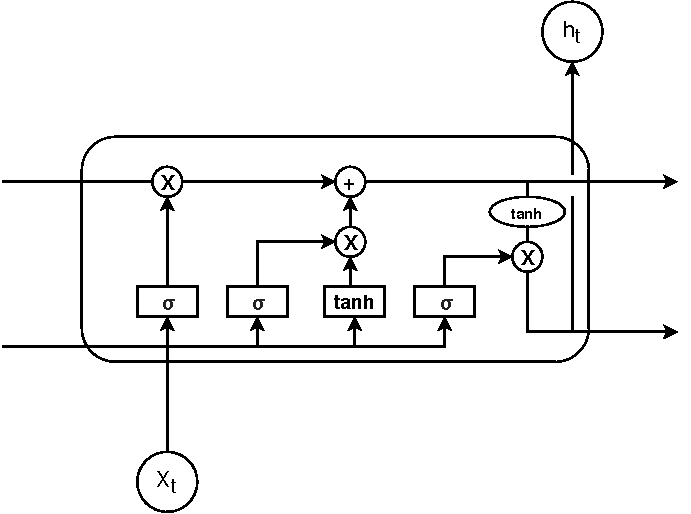
\includegraphics[width=0.5\textwidth]{figures/lstmCell.pdf}
  \caption{A cell in an LSTM network.}
  \label{lstm}
\end{figure}

LSTM networks are a special kind of RNN, which reduce the vanishing gradient problem. It makes them much more effective on capturing long-term dependencies. All recurrent neural networks have the form of a chain of repeating modules of neural network. LSTM network also has this chain structure, but the repeating module has a different structure. The key of the solution is usage of multiple gates and a cell state, which runs through all the cells and is manipulated using these gates – parts of the state may be added or removed. Each gate is a sigmoid layer that outputs a number between 0 and 1, which represents the degree of the cell state modification.

The Figure \ref{lstm} represents a structure of a LSTM cell. First, the network decides how much of information from previous steps to keep stored in its cell state, by using the forget gate, which consists of a sigmoid function applied to weighted sum of previous output, input and bias (equation \ref{eq:lstm_1}). $W$ are updated through the backpropagation algorithm weights, $b_f$ is a bias, $x_t$ is an input, $h_{t-1}$ is a hidden state from previous step.
\begin{equation} \label{eq:lstm_1}
f_t = \sigma(W_{xf}x_t + W_{hf}h_{t-1}+b_f)
\end{equation}

The next step is to decide how much of the inner state is going to be updated (i.e. what part of the result the cell is going to store in its state), by using input gate (equation \ref{eq:lstm_2}).
\begin{equation} \label{eq:lstm_2}
i_t = \sigma(W_{xi}x_t + W_{hi}h_{t-1}+b_i)
\end{equation}

After calculating the state modification, it is necessary to compute the new values (i.e. candidate values) which will be stored in it, by using activation function (equation \ref{eq:lstm_3}).
\begin{equation} \label{eq:lstm_3}
\tilde{c_{t}}=tanh(W_{xc}x_t + W_{hc}h_{t-1} + b_c)
\end{equation}

Updating the cell state is based on the previous state and the candidate values (equation \ref{eq:lstm_4}).
\begin{equation} \label{eq:lstm_4}
c_t = \tilde{c_{t}} \odot i_t + c_{t-1} \odot f_t
\end{equation}

Output gate is represented in equation \ref{eq:lstm_5}.
\begin{equation} \label{eq:lstm_5}
o_t = \sigma(W_{xo}x_t + W_{ho}h_{t-1}+b_o)
\end{equation}

And the final step producing the hidden state for the next timestep. It is based on the newly updated cell state, transformed by tanh function and multiplied by the output gate (equation \ref{eq:lstm_6}).
\begin{equation} \label{eq:lstm_6}
h_t = o_t \odot tanh(c_t)
\end{equation}

This model does not have a problem with vanishing gradient, but still the capacity of the LSTM memory is limited, because of inherently complex sequential words' paths from the previous unit to the current unit. The same complexity results in high computational requirements that make LSTM difficult to train. 

\section{Sequence-to-sequence model (seq2seq)} \label{seq2seq_section}

Seq2seq models were introduced by Google in 2014 \cite{sutskever2014sequence}. This model uses an encoder-decoder architecture (the Figure \ref{encoder_decoder}). Both the encoder and the decoder are recurrent neural networks (vanilla version of RNN is rarely used, because of the problems described in the section \ref{rnn_section}). The role of the encoder is to encode the input, a sequence of variable length data, to a fixed length vector. Decoder based on this vector generates an output sequence of data of different length. These 2 neural networks are connected into one model to maximize the learning effect. Seq2seq model is very effective to solve NLP problems, because input and output sequences can have different lengths and recurrent neural networks can work with context. This model is often used in machine translation, text summarization, dialogue systems etc.

\begin{figure}[hbt]
  \centering
  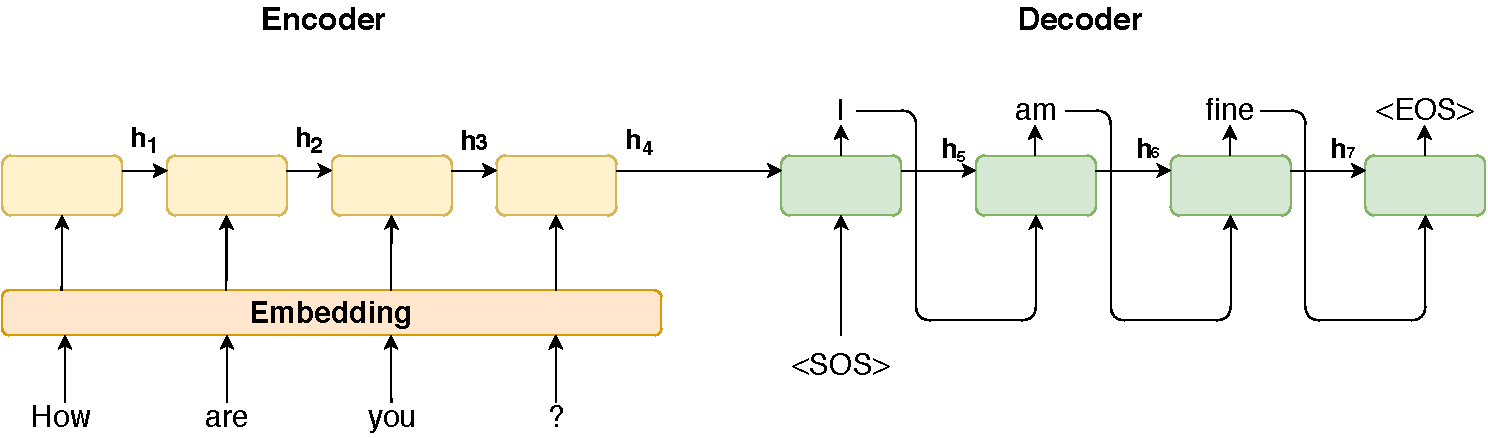
\includegraphics[width=0.8\textwidth]{figures/encoder_decoder.pdf}
  \caption{Architecture of sequence-to-sequence model.}
  \label{encoder_decoder}
\end{figure}

The Figure \ref{encoder_decoder} presents traditional encoder-decoder arhitecture. Encoder converts an input sequence of words to a corresponding fixed size hidden vector. Each vector represents the current word and the context of the word. Every time step, it takes a vector that represents a word and pass its output to the next layer. The last hidden state of encoder passes its output to the first layer of the decoder. The final hidden state of the encoder is also called context vector. The decoder input is an output encoder vector and start token, which characterizes the beginning of the generated sentence. The generated word depends on the previous decoder state and the last generated word. Many optimizations have led to other seq2seq components, such as attention, beam search, bucketing.

\section{Attention} \label{attention_section}
A neural attention mechanism is based on the human visual attention mechanism. Visual attention is able to focus on a certain region of an image with ``high resolution'', while perceiving the surrounding image in “low resolution”, and then adjusting the focal point over time.

In \cite{vaswani2017attention} attention is described as mapping a query and a set of key-value pairs to an output, where the query, keys, values, and output are all vectors. The output is computed as a weighted sum of the values, where the weight assigned to each value is computed by a compatibility function of the query with the corresponding key.

The attention mechanism provides the decoder with information from each hidden state of the encoder and it gives a model the ability to selectively focus on useful parts of the input sequence and learn the alignment between them (example in the Figure \ref{attention}).

\begin{figure}[hbt]
  \centering
  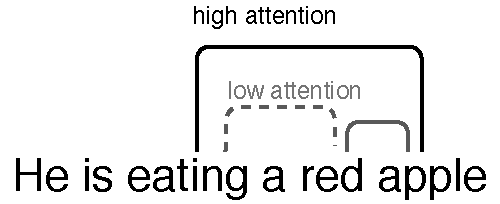
\includegraphics[width=0.5\textwidth]{figures/attention.pdf}
  \caption{When we see ``eating'', we expect to encounter a food word very soon. The color term describes the food, but probably not so much with ``eating'' directly.}
  \label{attention}
\end{figure}

Self-attention is an attention mechanism, where ``self'' means that the inputs interact with each other and ``attention'' means that inputs find out who they should pay more attention. Formally, in the attention mechanism the query, keys and values are from the same sequence. The query is a single element from the sequence while the keys and values are the entire sequence. The attention output is a new representation of the element that was the query. Self-attention is used to compute a new representation of the sequence.  

\section{Transformer} \label{sec_transformer}
Information in this section is taken from \cite{vaswani2017attention}.
\begin{figure}[hbt]
  \centering
  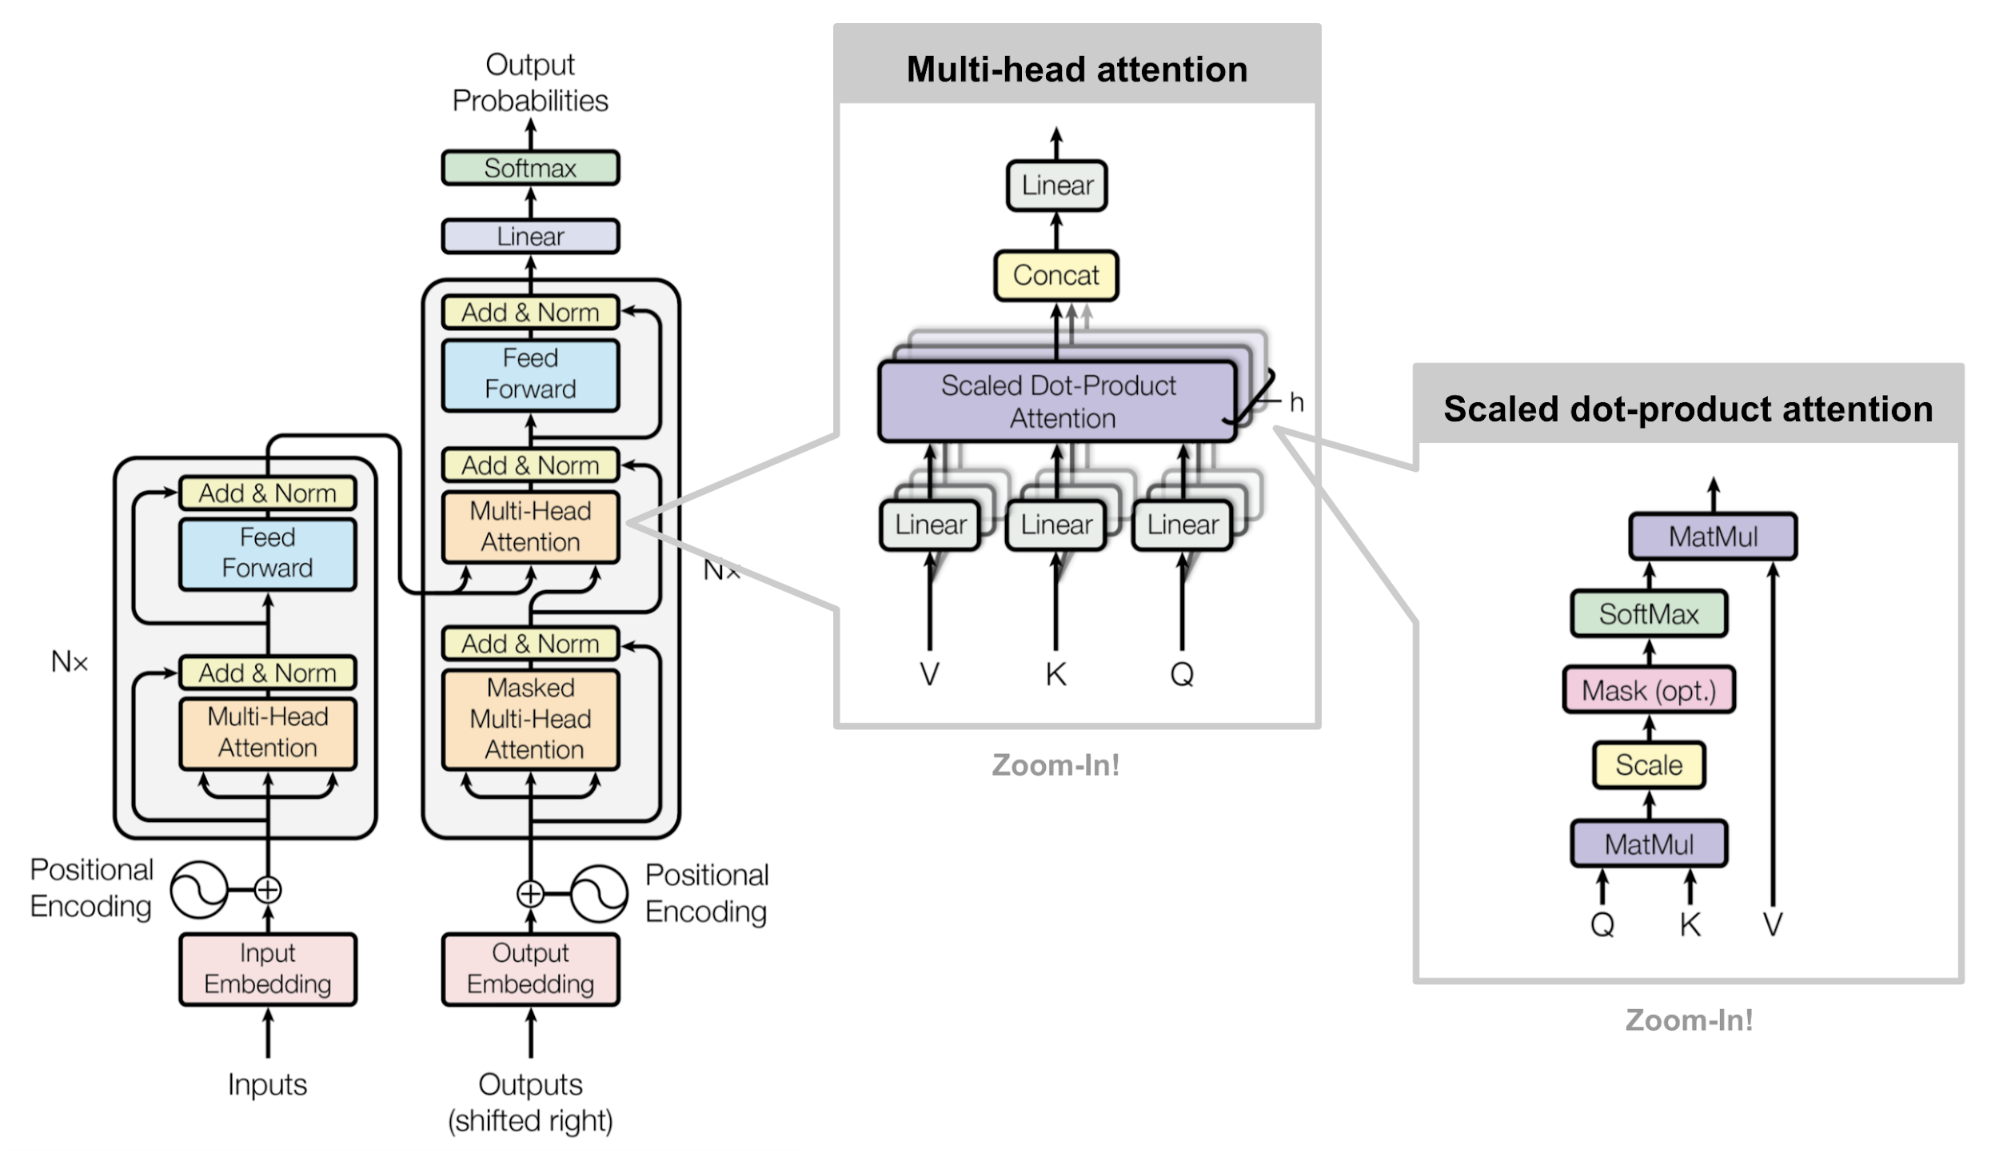
\includegraphics[width=0.9\textwidth]{figures/transformer_attention.png}
  \caption[Transformer architecture]{The architecture of the Transformer.\protect\footnotemark}
  \label{transformer}
\end{figure}

Transformer introduces an architecture that is based on self-attention mechanism and does not use any recurrent networks. In each step this model applies self-attention mechanism which directly models relationships between all words in a sequence, regardless of their respective position. Transformers do not require that the sentence be processed in order, that allows process parallelization during training, unlike RNN. Due to this feature, it has enabled training on much more data. 

The architecture of the Transformer is illustrated in the Figure \ref{transformer}. The Transformer consists of a stack of encoders (on the left) for processing inputs of any length and another set of decoders (on the right) to output the generated sentences. $N_x$ in the Figure means that modules of encoder and decoder can be stacked on top of each other multiple times. Modules consist of multi-head attention and feed forward layers. The inputs and output are first embedded into an n-dimensional space. Words' positions are added to the embedded representation, n-dimensional vector, of each word.
\footnotetext{\url{http://primo.ai/index.php?title=Transformer}}

\begin{equation} \label{eq:transformer_attention}
Attention(Q, K, V) = softmax(\frac{QK^T}{\sqrt{d_k}})V
\end{equation}

\begin{equation} \label{eq:transformer_multi_head}
MultiHead(Q, K, V) = Concat(head_1, head_2, ..., head_h)W^O
\end{equation}

An equation \ref{eq:transformer_attention} represents a \textbf{scaled dot-product attention}. The input consists of values of dimension $d_v$, queries and keys of dimension $d_k$, where queries, keys and values are matricies.

An equation \ref{eq:transformer_multi_head} represents a \textbf{multi-head attention}, which allows the model to jointly track information from different representation subspaces at different positions. Averaging inhibits this with a single head of attention. The input also consists of queries, keys and values matricies, $W^O$ is a parameter matrix, $h$ is a number of parallel layers, $head_i = Attention(QW_i^Q, KW_i^K, VW_i^V)$, where $W_i^Q, W_i^K, W_i^V$ are parameter matricies. $Q$, $K$ and $V$ are different for each position of the attention modules in the structure. It depends on if they are in the encoder, the decoder or between them.

\section{GPT} \label{sec_gpt}
Information in this section is taken from \cite{radford2018improving}.
GPT is a transformer-based (Section \ref{sec_transformer}) language model. The model works in 2 stages. First of all transformer model trained on a very large amount of data in an unsupervised manner (There are only input variables and no correspoding output variables in unsupervised dataset.), then the model is fine-tuned on much smaller supervised dataset (There are input and output variable in supervised dataset. The model learns the mapping function from the input to the output.) to help it solve specific tasks.

\subsubsection{Unsupervised pre-training}
In unsupervised pre-training a standard language modeling is used and the aim is to maximize the likelihood (Equation \ref{eq:unsupervised_pre_training}, where $U = {u_1, u_2, ... , u_n}$ is an unsupervised corpus of tokens, $k$ is the size of context window, $P$ is modeled using a neural network with parameter $\Theta$).

\begin{equation} \label{eq:unsupervised_pre_training}
L_1(U) = \sum_i \log P(u_i|u_{i-k}, ... , u_{i-1}; \Theta)
\end{equation}

Multi-layer Transformer decoder is used for the language model. The model applies a multi-headed self-attention operation over the input context tokens followed by position-wise feedforward layers to produce an output distribution
over target tokens (Equation \ref{eq:unsupervised_decoder}, where $U = (u_{-k}, ... , u_{-1})$ is the context vector of tokens, $n$ is the number of layers, $W_e$ is the token embedding matrix, $W_p$ is the position embedding matrix).

\begin{equation}  \label{eq:unsupervised_decoder}
\begin{array}{lcl} 
h_0 & = &UW_e + W_p \\

h_1 & = & transformer\_block(h_{l-1}) \forall l \in [1,n] \\

P(u) & = & softmax(h_n, W_e^T) \\
\end{array}
\end{equation}

\subsubsection{Supervised fine-tuning}
After training the model, the parameters are adapted to the supervised target task. Given a labeled dataset $C$, where an instance represents a sequence of input tokens $(x^1, ... , x^m)$, along with a label $y$. The inputs are passed through the pre-trained model to get the final transformer block's activation $h_l^m$, which is then fed into an additional linear output layer with $W_y$ parameters for predicting $y$ (Equation \ref{eq:supervised_fine_tune}). 

\begin{equation} \label{eq:supervised_fine_tune}
P(y|x^1, ... , x^m) = softmax(h_l^m, W_y)
\end{equation}

\begin{equation} \label{eq:supervised_maximize}
L_2(C) = \sum_{(x,y)} \log P(y|x^1, ... , x^m)
\end{equation}

Authors found that including language modeling as an auxiliary objective to the fine-tuning helped learning. First of all it improves the generalization of the supervised model. Secondly it accelerates convergence. They optimize the objective with weight $\lambda$ (Equation \ref{eq:objective_optimalization}).

\begin{equation} \label{eq:objective_optimalization}
L_3(C) = L_2(C) + \lambda * L_1(C)
\end{equation}

\section{BART} \label{bart_section}
BART is a denoising autoencoder for pretraining sequence-to-sequence models, that maps a corrupted document to the original document it was derived from. The model uses a standard Transformer-based neural machine translation architecture, with a bidirectional encoder and left-to-right decoder.

\begin{figure}[hbt]
  \centering
  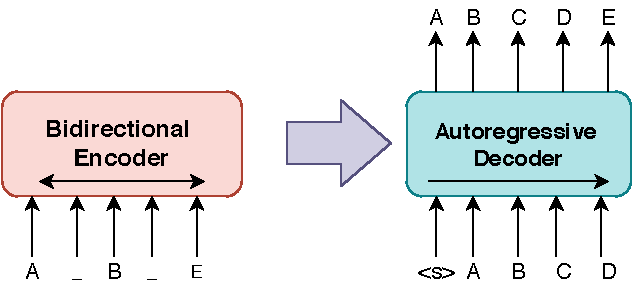
\includegraphics[width=0.6\textwidth]{figures/BART.pdf}
  \caption{BART: Inputs to the encoder need not be aligned with decoder outputs, allowing arbitary noise transformations. Here, a document has been corrupted by replacing spans of text with mask symbols. The corrupted document (left) is encoded with a bidirectional model, and then the likelihood of the original document (right) is calculated with an autoregressive decoder. For fine-tuning, an uncorrupted document is input to both the encoder and decoder, and we use representations from the final hidden state of the decoder\cite{lewis2019bart}.}
  \label{bart}
\end{figure}

Bidirectional encoder consists of $N$ transformer encoder blocks stacked on top of each other (Section \ref{sec_transformer}), the final block is the output. The input is a sequence of tokens, which are first embedded into vectors and the processed in the model. The output is a sequence of vectors of size $H$, in which each vector corresponds to an input token with the same index. Bidirectional encoder uses 2 training strategies: \textbf{Masked LM (MLM)} and \textbf{Next Sentence Prediction (NSP)}. 

In \textbf{MLM} 15\% of words in each sequence are replaced with a [MASK] token before embedding. The model then tries to predict the original value of the masked words, based on the context provided non-masked words in the sequence. Bidirectional encoder loss function takes into consideration only the prediction of masked values. Pretraining on this task allows the model to learn general features of the language.

\textbf{Next Sentence Prediction}. The bidirectional encoder in the training process receives pairs of sequences as input and the task of the model is to say whether the second sentence is a subsequent of the first sentence in the original document. During training, part of the inputs are a pair in which the second sentence is a subsequent in the original document and in the other part a random sentence from the corpus is chosen as the second sentence. The assumption is that the random sentence will be disconnected from the first sentence. Pre-training on this task allows the model to learn relationships between sentences.

\begin{eqfloat}
\begin{equation} \label{eq:relu}
f(x) = x^+ = max(0, x)
\end{equation}
\caption{Rectified Linear Unit (ReLU)}
\end{eqfloat}

\begin{eqfloat}
\begin{equation} \label{eq:gelu}
GELU(x) = xP(X \leq x) = x \Phi(x)
\end{equation}
\caption{Gaussian Error Linear Unit (GELU)}
\end{eqfloat}

\begin{eqfloat}
\begin{equation} \label{eq:gelu_approx}
\begin{array}{lcl} 
GELU(x) = 0.5x(1 + tanh[\sqrt{2/\pi}(x + 0.044715x^3)]) \\ 
GELU(x) = x\sigma(1.702x) \\
\end{array}
\end{equation}
\caption{Approximations of GELU}
\end{eqfloat}
Autoregressive decoder is GPT model (Section \ref{sec_gpt}). Authors modified ReLU activation functions (Equation \ref{eq:relu}) to GELU (Equation \ref{eq:gelu}) and initialized parameters from $\mathcal{N}(0, 0.2)$. Autoregressive decoder can be directly fine tuned for sequence generation tasks.

\begin{figure}[hbt]
  \centering
  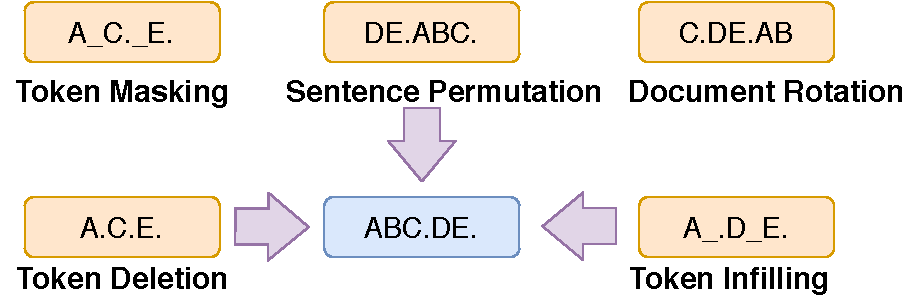
\includegraphics[width=0.6\textwidth]{figures/bart_doc_corruptions.pdf}
  \caption{Transformations for noising the input. These transformations can be composed.}
  \label{bart_doc_corruption}
\end{figure}

BART allows to apply any type of document corruption, such as token masking, sentence permutation, document rotation, token deletion, text infilling (Figure \ref{bart_doc_corruption}).

\chapter{Related works}
This chapter presents an overview of the most popular NLG models for building open-ended dialogue systems and for resolving problems described in the section \ref{nlg_ds_problems}. Section \ref{related_work_ds_section} presents approaches for resolving standard NLG problems. Section \ref{stylized_problems} presents solutions for generating stylized text, which helps to create the feeling that you are talking to a person.

\section{Approaches for dialogue systems problems} \label{related_work_ds_section}
Modeling conversations with generative probabilistic models was first proposed in \cite{ritter2011data}. They present a data-driven approach to generating responses to Twitter status posts, based on
phrase-based Statistical Machine Translation. In \cite{shang2015neural} authors proposed a framework for generating responses on micro-blogging websites with using recurrent neural networks. Their model can generate grammatically correct and content-wise appropriate responses to over 75\% of the input text.

\subsubsection{Text generation methods}
In the paper \cite{see2019makes} solutions to common NLG problems in dialogue systems described. Authors add control (the ability to specify desired attributes of the generated text at test time) and focus on four controllable attributes of text: repetition, specificity, response-relatedness and question-asking. They measure repetitiveness as n-gram overlap, specificity as word rareness, response-relatedness as the embedding similarity of the bot’s response to the human’s last utterance. In this work, authors use \textbf{Conditional Training (CT)} \cite{peng2018towards} and \textbf{Weighted Decoding (WD)} \cite{ghazvininejad2017hafez}. 

\begin{figure}[hbt]
  \centering
  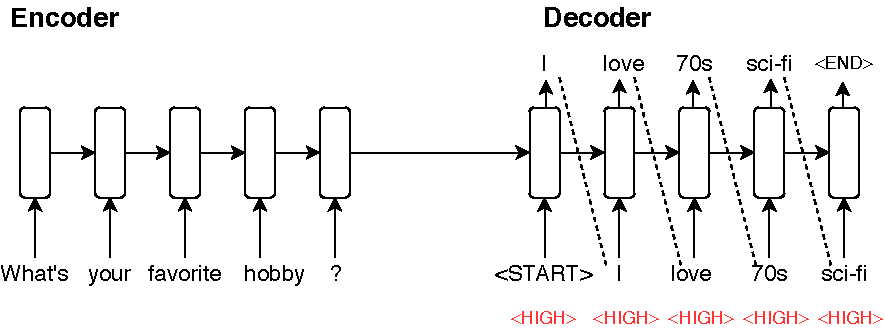
\includegraphics[width=0.7\textwidth]{figures/ct.pdf}
  \caption{Example of Condition Training model.}
  \label{ct}
\end{figure}


A \textbf{CT} model learns probabilities $P(y|x,z)$, where $y$ is the output text, $x$ is the input text and $z$ is a control variable, which specifies the desired output attribute. In the model $z$ is presented with learned embedding and is concatenated to each decoder input (the Figure \ref{ct}). For example, to get very generic or very specific response, $z$ can be set to LOW or HIGH. If it is necessary simultaneously control several attributes, multiple control embeddings ($z_1, z_2, ..., z_n$) can be concatenated and the model learns $P(y|x, z_1, z_2, ..., z_n)$. Disadvantage of Conditional Training is that it can’t control attributes without sufficient training data. CT model learns only a very weak connection between $z$ and the semantic relatedness of the output.

A \textbf{WD} is a technique applied during decoding to increase/decrease the probability of words with certain features. 
\begin{equation} \label{eq:wd}
score(w, y_{<t}; x) = score(y_{<t}; x) + \log P_{RNN}(w|y_{<t}, x) + \sum_i w_i * f_i(w; y_{<t}, x)
\end{equation}
In weighted decoding (Equation \ref{eq:wd}), a particial hypothesis $y_{<t} = y_1, ..., y_{t-1}$ is expanded by computing the score for each possible next word $w$ in the vocabulary on the $t^{th}$ step of decoding. $\log P_{RNN}(w|y_{<t}, x)$ is the log-probability of the word $w$ calculated by the RNN. $score(y_{<t}; x)$ is the accumulated score of the already-generated words in the hypothesis $y_{<t}$. $f_i(w; y_{<t}, x)$ is a decoding feature with associated weights $w_i$ (hyperparameters to be chosen). Each feature presents a specific controlling attribute.

\begin{equation} \label{eq:nidf}
NIDF(w) = \frac{IDF(w) - min\_idf}{max\_idf - min\_idf}
\end{equation}
\textbf{Normalized Inverse Document Frequency (NIDF)} is used as a measure of word rareness. In condition training the metric is represented as $z$ variable and in weighted decoding as a parameter of rareness for a word prediction (On each step of the decoding, the probability of each word in the vocabulary is updated in proportion to its rareness. The size of the update is controlled by a weight parameter.) (Equation \ref{eq:nidf}). $IDF(w) = \log(\frac{R}{c_w})$ is a Inverse Document Frequency of a word $w$, where $R$ is the number of responses in the dataset, $c_w$ is the number of those responses that contain $w$. $min\_idf$ and $max\_idf$ are the minimum and maximum IDF's, which are used for normalising the NIDF (ranges from 0 to 1).

Question-asking problem is resolved in CT by setting the variable $z$ to 1 of 11 possible values: $\{0, 1, ..., 10\}$, where $z=i$ means that the model should produce, on average, utterances containing ``?'' with probability $\frac{i}{10}$. In weighted decoding the binary decoding feature is used, which is equal to 1 if a word $w$ is in a pre-defined list of words: ``how, what, when, where, which, who, whom, whose, why, ?'', 0 otherwise.

N-gram based decoding features were defined to control repetition with WD. External (self-repetition across utterances), internal (self-repetition within utterances) and partner (repeating the conversational partner) repetition fetures identify repeating bigrams. Other features identify repeating content words. Negative weight is applied to these features to reduse repetition. 
\begin{equation} \label{eq:response_relatedness}
resp\_rel(w; y_{<t}, x) = cos\_sim(word\_emb(w), sent\_emb(l)) 
\end{equation}
Response-relatedness feature with weighted decoding is represented in the Equation \ref{eq:response_relatedness}, where $word\_emb(w)$ is the GloVe embedding for the word $w$, $sent\_emb(l)$ is the sentence embedding for the partner's last utterance $l$ ($l$ is part of the context $x$), $cos\_sim$ is the cosine similarity between two.
The control response-relatedness in condition training is represented by variable $z$ as $cos\_sim(sent\_emb(y), sent\_emb(l))$, where $cos\_sim$ is a cosine similarity between the model's response $y$ and the partner's last utterance $l$.

\subsubsection{Decoding strategies}
According to \cite{holtzman2019curious} decoding strategies with likelihood maximazing lead to text that is increadibly degenerate, even when using state-of-the-art models. If the most likely word is always sampled, the model generates repetitive and overly generic text, like ``I don't know'', because it is a typical answer to any question.

Maximization-based decoding methods such as \textbf{beam search} make text incoherent and repetitive. A beam search is a limited-width breadth first search. This method starts from an empty sequence $(t=0)$, at every step $t=0, 1, 2, 3,...$ beam search expands at most $k$ partial sequences (with highest probabilities) and computes the probabilities of sequences with length $t+1$. It terminates with a beam of $k$ complete sequences. 

Popular sampling methods for generation texts are based on sampling from the distribution. Temperature and top k sampling are the most popular methods to combat sampling from the tail.

\textbf{Temperature sampling} is inspired by statistical thermodynamics, where high temperature means low energy states are more likely encountered. In a probability model logits are divided by the temperature, before feeding them into softmax (Equation \ref{eq:temperature_sampling}, where $t$ is a temperature, $u_{1:|V|}$ are logits). Setting $t \in [0,1)$ skews the distribution towards high probability events, which implicitly lowers the mass in the tail distribution. The temperature parameter controls the shape of distribution without sufficiently suppressing the unreliable tail.

\begin{equation} \label{eq:temperature_sampling}
p(x=V_l|x_{1:i-1}) = \frac{exp(u_l / t)}{\sum_{l'} exp(u_l' / t)}
\end{equation}

\textbf{Top-k sampling} means sorting by probability and probabilities for anything below the token $k$ are set to 0. But in some cases, there are few words to choose, there is a risk of generating bland or generic text, while if $k$ is large the top-k vocabulary will include inappropriate candidates which will have their probability of being sampled increased by the renormalization. The top-k vocabulary $V^{(k)} \subset V$ (the set of size $k$) maximizes $p' = \sum_{x \in V^{(k)}} P(x|x_{1:i-1})$. The distribution is then re-scaled as in Equation \ref{eq:top_K_sampling}.

\begin{equation} \label{eq:top_K_sampling}
P'(x|x_{1:i-1}) = \begin{cases} 
          P(x|x_{1:i-1}) / p' & \mbox{if $x \in V^{(k)}$} \\
          0 & \mbox{otherwise}\\
         \end{cases}
\end{equation}

The research shows how different natural distribution of human texts and the distribution of machine text produced from maximum likelihood decoding. To resolve this problem authors introduced \textbf{Nucleus Sampling}. The concept is that the vast majority of probabilities are concentrated in a small subset (\textit{nucleus}) of the vocabulary that tends to vary from one to a few hundred candidates. Sampling from the top-$p$ portion of the probability mass expands and contracts the candidate pool dynamically. Formally, given a distribution $P(x|x_{1:i-1}$, the top-p vocabulary $V^{(p)} \in V$ is defined to satisfy the condition in the Equation \ref{eq:nucleus_sampling}.

\begin{equation} \label{eq:nucleus_sampling}
\sum_{x \in V^{(p)}} P(x|x_{1:i-1})  \geqslant p
\end{equation}

\section{Approaches for generating stylized conversation} \label{stylized_problems}
The idea that computers can generate stylized texts appeared half a century ago in \cite{wheatley1965computer}. Authors choose a variety of text characteristics as style, such as an expession of politeness in machine translation \cite{sennrich2016controlling}, transformation from modern English to Shakespearean English \cite{jhamtani2017shakespearizing}, sentiment of a text in \cite{shen2017style} and \cite{li2018delete}. In \cite{gao2019structuring} authors used a structured latent space to generate stylized dialogue responses. Another approach was proposed in \cite{john2018disentangled}, where authors applied an adversarial loss to separate style from content. The problem of style transfer, described in these papers, differs from the stylized text generation, because as it is shown in \cite{guu2018generating} an existing human-written source used to control the reliability of the results can significantly improve the quality of the resulting texts. 

\subsubsection{ECM}
Emotional Chatting Machine (ECM), represented in \cite{zhou2018emotional}, can generate not only relevant and grammatical responses, but also emotionally consistent. This framework proposes seq2seq architecture. This separate responses into several categories (Angry, Disgust, Happy, Like, Sad, Other). The emotion category of the to-be-generated response is given for ECM, because, in the opinion og the authors, emotions are highly subjective. 

\begin{figure}[hbt]
  \centering
  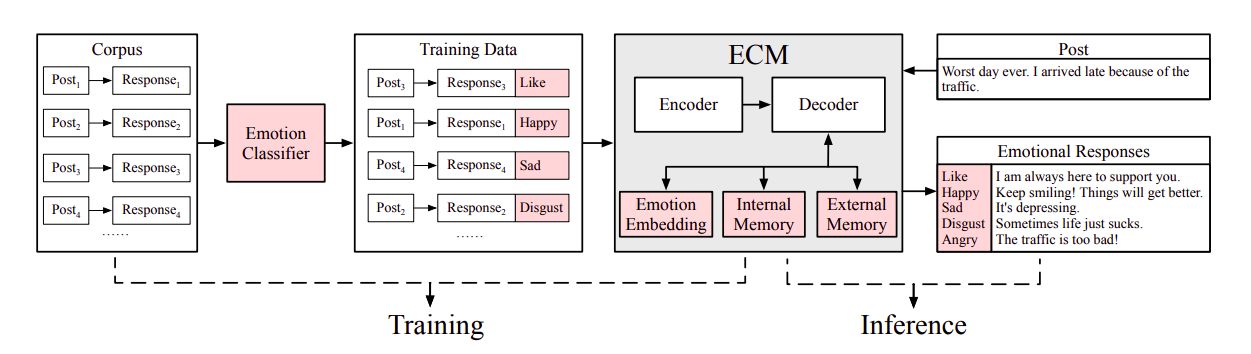
\includegraphics[width=1\textwidth]{figures/ecm.png}
  \caption{ Overview of ECM (the grey unit). The pink units are used to model emotion factors in the framework.}
  \label{ecm}
\end{figure}

In the architecture (the Figure \ref{ecm}) a post can be answered with different emotions, depending on the attitude of the respondent. For example, for a sad story, someone may respond with anger  (as an irritable stranger), sympathy (as a friend) or happy (as an enemy). \textbf{Emotion classifier} generates labels for each response. Generated labels and responses are fed into ECM to generate emotional responses conditioned on different emotion categories. In \textbf{Emotion Category Embedding} randomly initialize the vector of an emotion category $v_e$ for each category $e$. During the training the model is learning the vectors of the emotion category. \textbf{Internal memory} captures emotion dynamics during decoding. It is achieved using the following concept: before the decoding process each category has an internal emotion state; at each step the emotion state decays by a certain amount; when decoding process is completed, the emotion state should be zero, what indicates that the emotion is completely expressed. \textbf{External memory} is used to model emotion expressions explicitly, the model can choose to generate words from  an emotion vocabulary or a generic vocabulary.

ECM need an external decision maker, because this model has to specify an emotion category to be generated.

\subsubsection{Generation of stylized texts}

In the paper \cite{tikhonov2018guess} authors describe the problem of stylized text generation in a multilingual setup and show the importance of phonetics for generating the author's stylized poetry. They presented a version of a language model based on a LSTM artificial neural network with extended phonetic and semantic embeddings for stylized poetry generation. The model generates texts resembling the writing style of a particular author.

\begin{equation} \label{eq:poetry_nlg}
G(C|S) = \begin{cases} 
          (C, \mathbb{R}^m, F) \rightarrow \{T_i^G\} \\
          \{T_i^G|S\}  \mathtt{\sim}  \{T_i|S\} & \mbox{w.r.t. D}\\
         \end{cases}
\end{equation}

The equation \ref{eq:poetry_nlg} represents the stylized model, where $C = \{ T_i\}^M_{i=0}$ is a corpus of $M$ literary texts written in one natural language. Every text of length $l$ is a sequence $T_i = (w_j)^l_{j=0}$ ($w_j$ is a word). Words are drawn from a vocabulary set $V = \{ w_j \}^L_{j=1}$, $L$ is a vocabulary size. $(C, \mathbb{R}^m, F)$ is all information available to us.

Performance metric $D$ usually tries to minimize $D(\{T_i\}, \{T_i^G\})$, where $\{T_i^G\}$ is a randomized sample of $C$. $S$ is a subset of continuous and categorical variables out of $(\mathbb{R}^m, F)$ and metric $D$. Artificial neural networks are used for language modeling to avoid the dimensionality curse by effective mapping $(C,\mathbb{R}^m, F) \rightarrow \mathbb{R}^d$ and then train the model like that $G(C):\mathbb{R}^d \rightarrow \{ T_i^G\}$. 

Advantage of this model is a customization. To control cetain parameters of the model, it is needed to include them intp $S$. The output $\{T_i^G|S\}$ will resemble original texts $\{T_i|S\}$ that satisfy $S$ conditions. The name of an author of a poetic text is used as a condition $S$ for the model. 

Another key feature of the proposed model is a concatenated word representation, where one of the LSTMs works with letters from char-representation of the word and another one uses phonemes of the International Phonetic Alphabet, employing an heuristics to transcribe words into phonemes.
 
\chapter{Evaluation methods and datasets}
The majority of NLG researches published between 2005-2014 relies on automatic metrics \cite{gkatzia2015snapshot}. A lot of NLG evaluations use automatic metrics, because it is a cheap and fast method. These metrics are reasonable if they are known to be enough correlated with human preferences. According to \cite{artstein2009semi} conversational dialogue systems cannot be evaluated by automatic metrics, because dialogue is heavily dependent on context and theory of current dialogue is not precise enough to predetermine the target output.  

Metrics METEOR, BLEU, ROUGE are usually used for automatic summarization. They assume that valid responses have significant word overlap with the ground truth responses. In dialogue systems these metrics cannot be used, because there is significant diversity in the space of valid responses to a given context \cite{liu2016not}.

In the paper \cite{novikova2017we} the weak correlation between human and automatic evaluations is also confirmed. Authors compared different word-based (\textbf{WBM} relies on ground-truth references) and grammar-based (\textbf{GBM} does not rely on ground-truth references) metrics. Their model, combination of WBMs and GBMs, achieved high correlation with humans but only within a single domain.

Corpus is very important for successful Natural Language Generation. Dialogue systems require training data in the format of people text conversation, for example, non-fiction or movie reviews are not suitable for this. Large volumes of training data improves the decision-making ability of NLG model, so those models can use it to figure out patterns. Quality is more important for training data than the quantity of data points. Unfortunately, there are not a lot of datasets available for training NLG models, due to the high cost of creating quality datasets. 

In my bachelor thesis I am using 2 different dataset (Twitter data and Persona-Chat). 

\subsection{Persona-Chat dataset} \label{persona_chat_subsec}

\begin{table}[ht]
  \begin{tabular}{ |c|c| }
   \hline\hline
   \textbf{Persona 1} & \textbf{Persona 2}  \\ 
   \hline\hline
    I like to ski. & I am an artist. \\
    My wife does not like me anymore. & I have four children. \\
    I have went to Mexico 4 times this year. & I recently got a car. \\
    I hate Mexican food. & I enjoy walking for exercise. \\
    I like to eat cheetos. & I love watching Game of Thrones. \\
    \hline\hline
    \multicolumn{2}{l}{[PERSON 1:] Hi} \\
    \multicolumn{2}{l}{[PERSON 2:] Hello! How are you today?} \\
    \multicolumn{2}{l}{[PERSON 1:] I am good thank you, how are you.} \\
    \multicolumn{2}{l}{[PERSON 2:] Great, thanks! My children and I were just about to watch Game of Thrones.} \\
    \multicolumn{2}{l}{[PERSON 1:] Nice! How old are your children?} \\
    \multicolumn{2}{l}{[PERSON 2:] I have four that range in age from 10 to 21. You?} \\
    \multicolumn{2}{l}{[PERSON 1:] I do not have children at the moment.} \\
    \multicolumn{2}{l}{[PERSON 2:] That just means you get to keep all the popcorn for yourself.} \\
    \multicolumn{2}{l}{[PERSON 1:] And Cheetos at the moment!} \\
    \multicolumn{2}{l}{[PERSON 2:] Good choice. Do you watch Game of Thrones?} \\
    \multicolumn{2}{l}{[PERSON 1:] No, I do not have much time for TV.} \\
    \multicolumn{2}{l}{[PERSON 2:] I usually spend my time painting: but, I love the show.} \\
    \hline\hline
  \end{tabular}
  \caption{Example of a dialogue from the Persona-Chat dataset \cite{zhang2018personalizing}.}
\label{tab:persona_chat}
\end{table}

\begin{table}[t]
\centering
  \begin{tabular}{ |c|c| } 
   \hline\hline
   \textbf{Original Persona} & \textbf{Revised Persona}  \\ 
   \hline\hline
   I love the beach. & For me, there is nothing like a day at the seashore. \\ 
   My dad has a car dealership. & My father sales vehicles for a living.  \\
   I just got my nails done. & I love to pamper myself on a regular basis. \\
   I am on a diet now. & I need to lose weight. \\
   Horses are my favorite animal. & I am into equastrian sports. \\ 
   \hline
  \end{tabular}
  \caption{Example of original and revised personas \cite{zhang2018personalizing}.}
\label{tab:persona_revised}
\end{table}

\begin{table}[t]
\centering
  \begin{tabular}{|p{8cm}|p{2cm}|} 
  \hline
  Average number of words in first persona description: & 6.332 \\
  \hline
  Average number of words in second persona description: & 6.321 \\
  \hline
  Average number of words in the first person's utterances: & 11.419 \\
  \hline
  Average number of words in the second person's utterances: & 11.929 \\
  \hline
  Number of first persona description's sentences: & 40239 \\
  \hline
  Number of second persona description's sentences: & 40126 \\
  \hline
  Number of the first person's utterances: & 65719 \\
  \hline
  Number of the second person's utterances:  & 65719 \\
  \hline
  Number of dialogues & 8938 \\
  \hline
  \end{tabular}
  \caption{Persona-Chat statistics.}
\label{tab:persona_chat_statistics}
\end{table}

Persona-Chat models normal conversation when 2 people meet for the first meet and try to get know each other better. The aim of the dialogue is to learn about interests of another person, find common ground and discuss their hobbies. The task involves both asking and answering questions. 

Persona-Chat dataset consists of small conversations between 2 crowdworkers from Amazon Mechanical Turk who were randomly paired and asked to act the part of a given provided persona (randomly assigned, and created by another set of crowdworkers). The data collection consists of persona chat (each dialogue has 6-8 turns), personas (set of 1155 possible personas, each consisting of at least 5 profile sentences), revised personas to avoid word overlap, because crowdworkers sometimes could repeat profile information in a chat(the Table \ref{tab:persona_revised}). In turn-based dialogue each message consists of a maximum of 15 words. All statistics are presented in the Table \ref{tab:persona_chat_statistics}, the Figure \ref{fig:histogram_persona_desc} and the Figure \ref{fig:histogram_uttr_length}. An example of Persona-Chat dialogue is shown in the Table \ref{tab:persona_chat}. The dataset contains 262,848 message-responses pairs and splitted into train data - 70\%, valid data - 20\% and test data - 10\%.

\subsection{Datasets for stylisation and pretraining} \label{stylistic_dataset_section}
\textbf{Stanford Sentiment Treebank (SST)} contains sentences from movie reviews and includes labels for every syntactically plausible phrase in thousands of sentences. To create SST the corpus of movie review excerpts from the paper \cite{pang2005seeing} is used, where HTML tags and sentences that are not in English are deleted from this dataset. The Stanford Parser is used to parse all 10,662 sentences and some snippet were splitted into multiple sentences. The resulting 215,154 phrases were labeled by Amazon Mechanical Trunk. There are 25 different labels from \textit{very negative} to \textit{very positive}. Annotators most often used only 5-class classification: negative, somewhat negative, neutral, positive or somewhat positive. Many of sentences could be considered neutral, therefore, to generate text with positive and negative sentiment I have used negative and somewhat negative classes as one negative class and positive, somewhat positive classes as one positive class. A histogram for SST is represented in the Figure \ref{fig:sst}.

For poetic style the Shakespeare dataset was used, which contains all of Shakespeare's plays. A histogram for this dataset is shown in the Figure \ref{fig:shakespeare}.

\begin{table}[ht]
\centering
 \begin{tabular}{|p{4cm}|p{3cm}|p{3cm}|} 
 \hline\hline
 reddit\_jokes.json & 195K jokes & 7.40M tokens \\
 \hline
 stupidstuff.json & 3.77K jokes & 396K tokens \\
 \hline
 wocka.json & 10.0K jokes & 1.11M tokens \\
 \hline\hline
 TOTAL & 208K jokes & 8.91M tokens \\
 \hline\hline
 \end{tabular}
 \caption{Statistics of jokes' dataset}
\label{tab:jokes}
\end{table}


A dataset of english plaintext jokes was used for generating funny text. There are about 208 000 jokes scraped from 3 sources (Table \ref{tab:jokes}). stupidstuff.json is scrapped from stupidstuff.org, wocka.jsom from \url{http://wocka.com}, reddit\_jokes.json is scraped from \url{https://www.reddit.com/r/Jokes} and contains all submissions to the subreddit as of 13.02.2017. A histogram for the dataset is shown in the Figure \ref{fig:jokes}.

Twitter dataset contains 867,710 message-response pairs from Twitter and is used for pretraining baseline model. The dataset is splitted into train data - 85\%, valid data - 10\% and test data - 5\%. A histogram for the dataset is shown in the Figure \ref{fig:tweet}


\chapter{Implementation, experiments and evaluations}
This chapter describes the model for stylized text generation, performed experiments and evaluation of the model results. The designed architecture is represented in the Figure \ref{architecture_nlg} and implemented in 2 variant. The first variant uses LSTM-based models and the second variant uses transformer-based pretrained models. All parts of the architecture were implemented in Python 3.7.3 with using PyTorch 1.4.0 framework.

\begin{figure}[hbt]
  \centering
  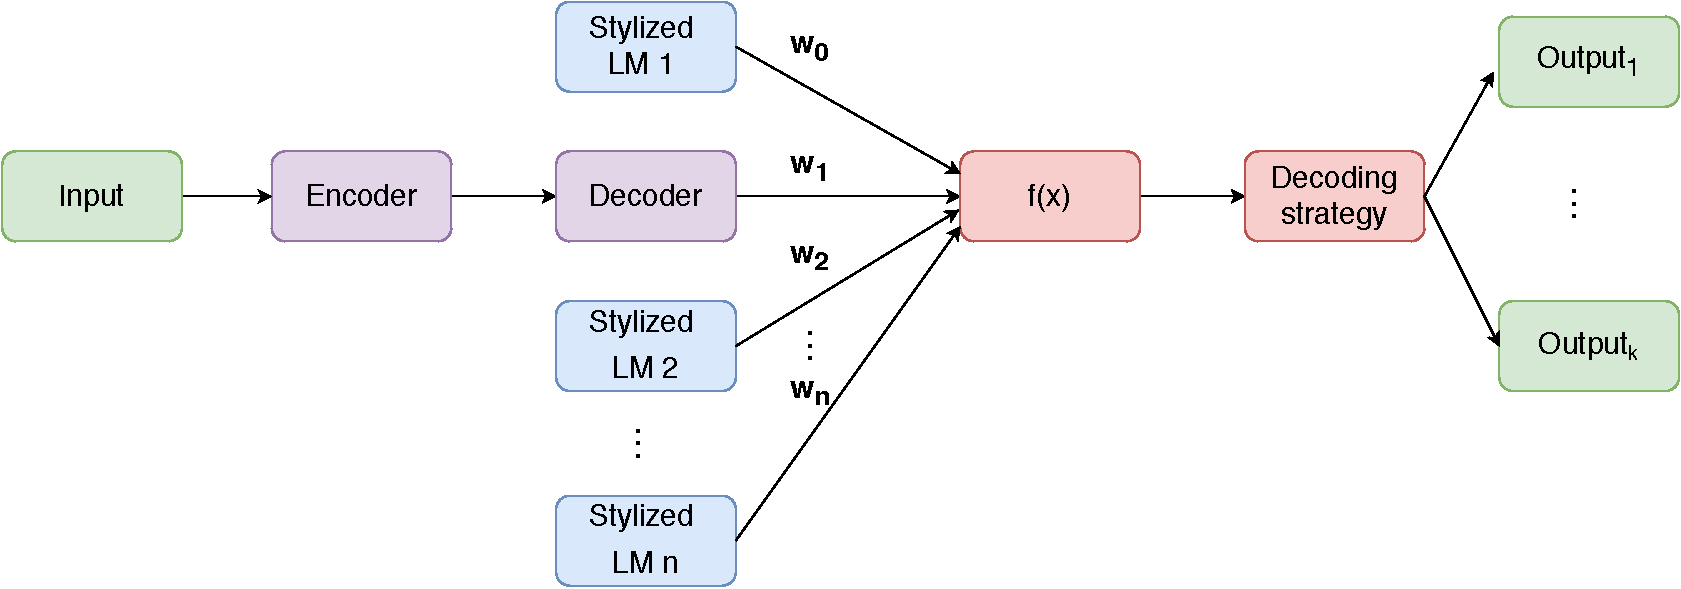
\includegraphics[width=0.7\textwidth]{figures/model.pdf}
  \caption{An architecture of stylized Natural Language Generation model.}
  \label{architecture_nlg}
\end{figure}

Encoder-Decoder model was trained on the Persona-Chat dataset, described in the subsection \ref{persona_chat_subsec}. As the input $x$ to the encoder-decoder model, the entire dialogue history, separated by unique token, is used. Each stylized language model was trained separately on the corresponding stylistic dataset described in the subsection \ref{stylistic_dataset_section}. Data are tokenized, where tokenization is a process of splitting text into units represented at model's input and replacing sensitive data with unique identification symbols that retain all the essential information about the data without compromising its security. Spacy\protect\footnotemark library is used with few handcrafted rules for tokenization.

\footnotetext{\url{https://spacy.io/}}

During the testing phase beam search, nucleus and temperature samplings were used to generate more varied answers. These decoding methods are described in detail in the section \ref{related_work_ds_section}.

\section{Baseline}
Encoder-decoder model in baseline is implemented as LSTM sequence-to-sequence language model with Luong attention and stylized language model is implemented as LSTM-based RNN model. LSTM neural networks are described in detail in the section \ref{lstm_section}, seq2seq model is described in the section \ref{seq2seq_section} and Luong attention is described in the appendix \ref{luong_attn_appendix}.

GloVe (Global Vectors) model was used for distributed word representation \cite{pennington2014glove}. It is an algorithm, which maps words into a meaningful space where the distance between words is related to semantic similarity. The model was trained only on the nonzero elements in a word-word cooccurrence matrix.


\begin{figure}[hbt]
  \centering
  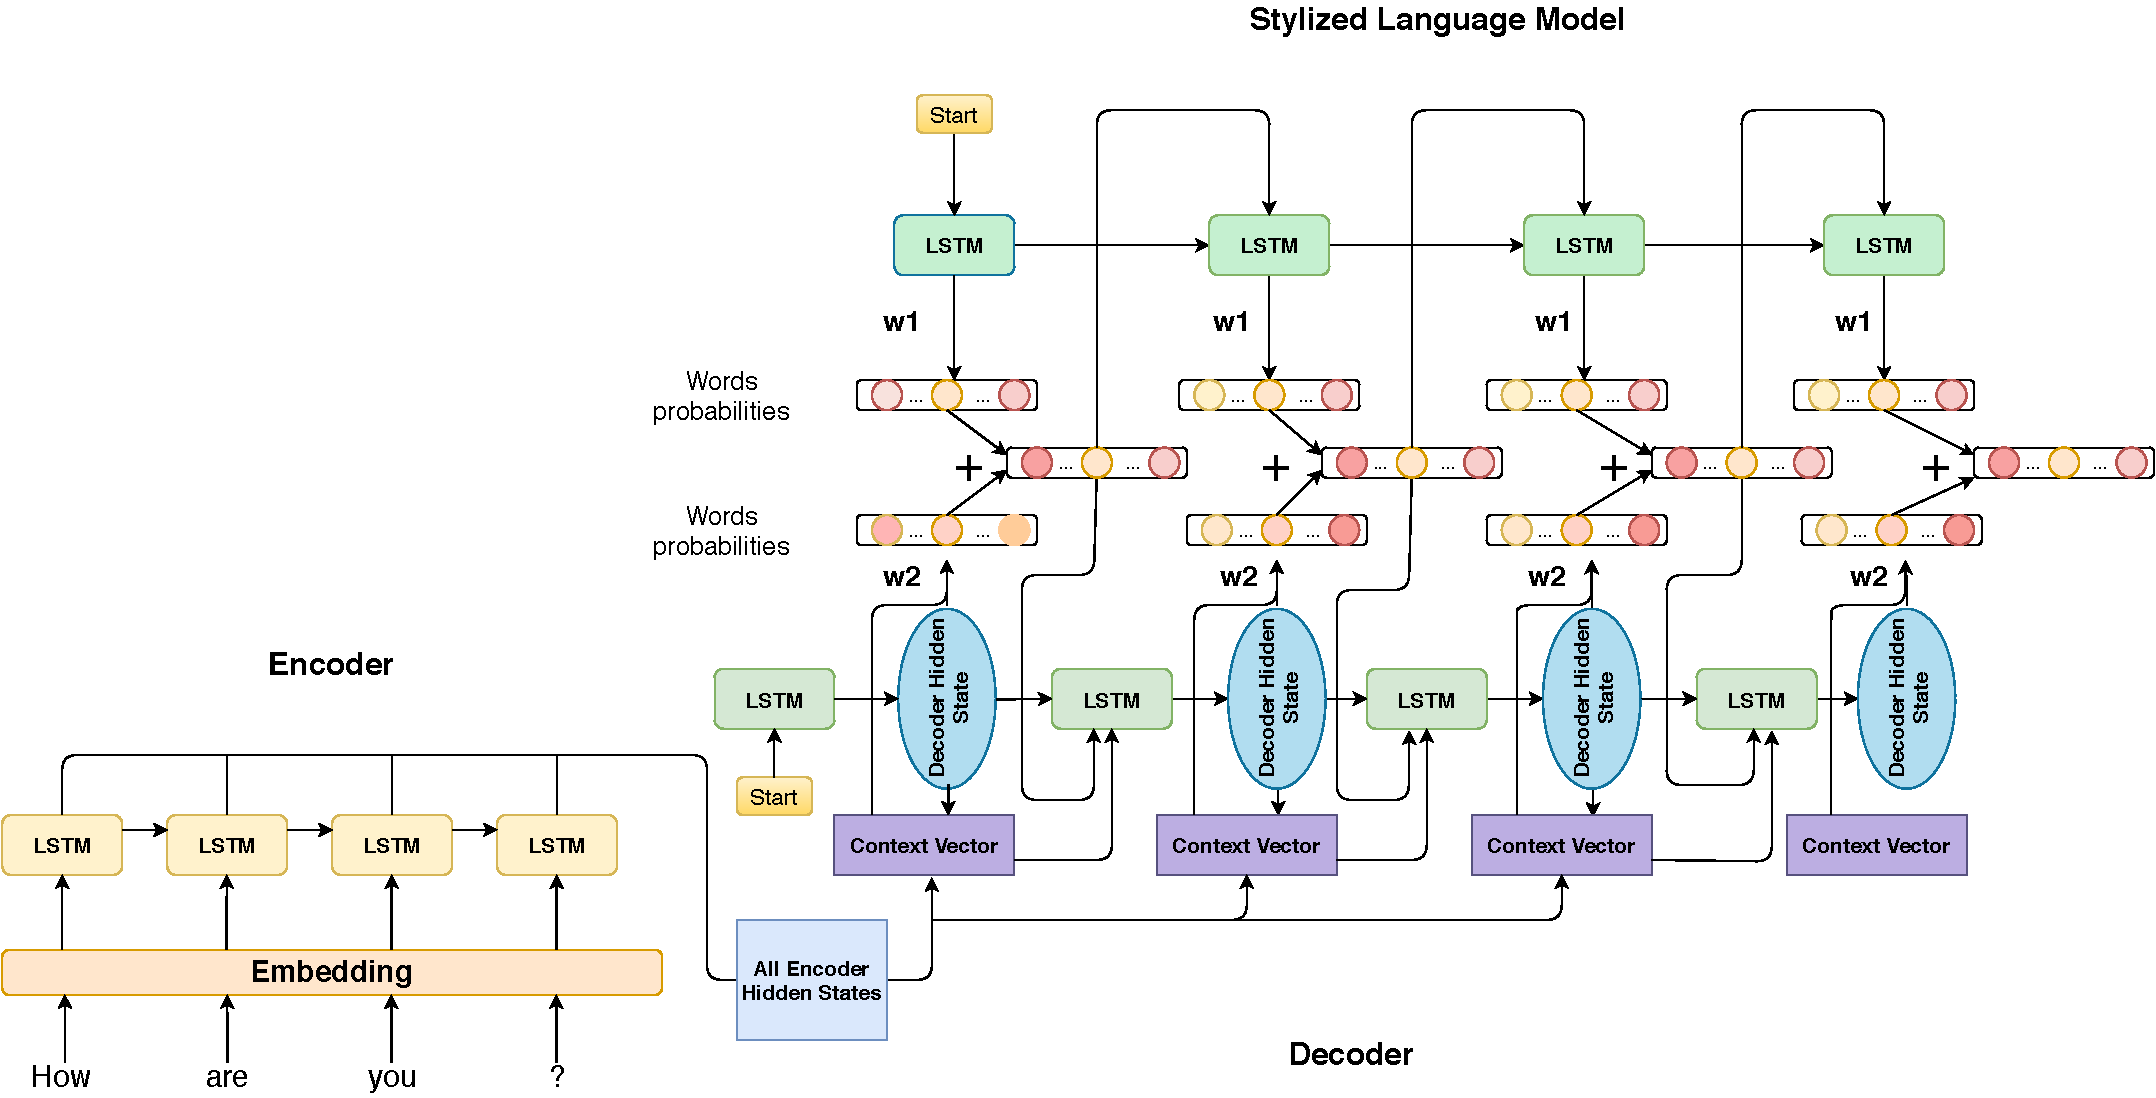
\includegraphics[width=1\textwidth]{figures/combine_models.pdf}
  \caption{Stylized Natural Language Generation baseline model.}
  \label{implementation_architecture}
\end{figure}

For all experiments with the baseline 2 hidden layers were used in both the encoder and decoder with 512 hidden unites in each hidden layer. A dropout \cite{srivastava2014dropout} was used with the probability of $50\%$ to prevent neural networks from overfitting. \textit{Cross-entropy} (measure of the difference between 2 probability distributions for a given random variable or set of events) was used as a loss function. Formally representation of cross-entropy is in the Equation \ref{eq:cross_entropy}. \textit{Adam} \cite{kingma2014adam} is used as the optimization algorithm.

\begin{eqfloat}
\begin{equation} \label{eq:cross_entropy}
H(p,q) = -\sum_{x \in X} p(x)\log(q(x))
\end{equation}
\caption{$p$ is the target distribution, $q$ is the approximation of the target distribution. $p(x)$ is the probability of the event $x$ in $p$, $q(x)$ is the probability of the event $x$ in $q$.}
\end{eqfloat}

\section{Pretrained models}
BART and GPT-2 models are used to explore all features of the created architecture (the Figure \ref{architecture_nlg}). GPT-2 is a successor to GPT, described in the section \ref{sec_gpt} and used as stylized language model. GPT-2 is a direct scale-up of GPT, with more parameters (1.5 billion parameters) and trained on more amount of data. It is a large transformer-based language model, which was trained to predict the next word in 40GB of Internet text. 

BART is an autoencoder for pretraining sequence-to-sequence models, described in the section \ref{bart_section}. BART decoder is a GPT model. GPT-2 model uses more words in a vocabulary than GPT, what means that before a combination of these models, it is necessary to convert a distribution of probabilities of the next word in a sequene over all the words in the smallest vocabulary to the distribution over the biggest one and add 0 if word does not exist. 

\section{Experiments}
\subsection{Experiment \#1: NIDF}
The first experiment was with Normalized Inverse Document Frequency as a decoding feature, described in the section \ref{related_work_ds_section}. This approach makes generated text more specific, because the less often a word is found in a dataset the more weight is setted for the word probability. 

The example with Baseline model, represented in the Table \ref{tab:baseline_experiment}, shows a repetition problem, such as repetition of the part of an utterance (``I am''), repetition of phrases (``I am afraid''). Another problem is that very often expressions do not make sense in the context. These problems can be because of the small amount of data and LSTM neural networks still has a problem to hold a context. To solve it, I have used transformer-based pretrained models.

Example of the generated dialogue is shown in the Table \ref{tab:compare_nidf}.

\subsection{Experiment \#2: Weighted decoding with using BART and GPT-2 models}
\begin{equation} \label{eq:baseline}
p(y_1, ... , y_{T'}|x_1, ... , x_T) = \prod_{t=1}^{T'} ( w_1 * p_1(y_t|v, y_1, ... , y_{t-1}) + \sum_{i=2}^n w_i * p_i(y_t| y_1, ... , y_{t-1}))
\end{equation}

The Equation \ref{eq:baseline} is a formal description of the experiment with weighted decoding, where $x_1, ... , x_T$ is an input sequence and $y_1, ... , y_{T'}$ is its corresponding output sequence whose length $T'$ may differ from $T$. $p_1(y_t|v, y_1, ... , y_{t-1})$ is a distribution for encoder-decoder language model, in which $v$ is the last hidden state of the encoder. $p_i(y_t|v, y_1, ... , y_{t-1})$ is a distribution for each stylized language model, $n$ is a number of stylized models. All distributions are represented with a softmax over all the words in the vocabulary and multiplied by a corresponding weight $w$, a hyperparameter to be chosen. 

Examples represented in the Tables \ref{tab:bart_conversation_gpt2}, \ref{tab:poetic_shakespear}, \ref{tab:sst_wd} shows the generated stylized dialogues with using stylistic datasets. 

In the Table \ref{tab:sst_wd} GPT-2 is trained on SST dataset. As a result generated sentences are short. It could be because sentences in the courpus are ranging from 10 to 20 words (a histogram of the SST dataset is in the Figure \ref{fig:sst}).

\subsection{Experiment \#3: Generating sequences by switching BART and GPT-2 models}
In this experiment $n$ words in a sequence are generated over BART and $n$ words are generated over GPT-2 model, where $n$ is a hyperparameter. Sequence generation stops when the end mark of the sequence is generated or the length of the sequence is equal to the maximum length.

Examples of this experiment are represanted in the Tables \ref{tab:jokes_switch} \ref{tab:shakespeare_switch}, \ref{tab:sst_switch}.

\subsection{Experiment \#4: Generating sequences by Nucleus sampling and Beam search}
In this experiment the results of the generated sequences by 2 different decoding methods are represented. All these decoding strategies are described in detail in the section \ref{related_work_ds_section}.

\begin{table}[ht]
\centering
 \begin{tabular}{|p{14cm}|} 
 \hline\hline
 hi , how it goes \\
 \hline
 i love you. \\
 \hline
 i do not love you. What do you mean? \\
 \hline 
 i am very glad you came to England \\
 \hline 
 that sounds like a good man \\
 \hline 
 i have not heard of you yet. \\
 \hline 
 i have been, i have been. You are welcome, sir \\
 \hline\hline
 \end{tabular}
 \caption{Experiment of Beam search decoding method}
\label{tab:beam_search}
\end{table}

\begin{table}[ht]
\centering
 \begin{tabular}{|p{14cm}|} 
 \hline\hline
  hi, how is thy name \\
 \hline
  i am an ass, and thou shalt be \\
 \hline
  i am sure you have not seen a man till you \\
 \hline 
  i do not know, Wherefore you speak. \\
 \hline 
 i ride you, And i love it \\
 \hline 
 i am very glad you are come \\
 \hline 
 i have a daughter of old \\
 \hline\hline
 \end{tabular}
 \caption{Experiment of Nucleus sampling decoding method}
\label{tab:nucleus_sampling}
\end{table}

\chapter{Conclusion}
The goal was to create a model that generates a stylistic response to the utterance of an opponent in the dialogue. 

